% arara: pdflatex: { shell: yes }
% arara: pdflatex: { synctex: true, shell: yes }
%
\documentclass{beamer}

\mode<presentation>
{
  \usetheme{Madrid}
  \setbeamercovered{transparent}
  \useinnertheme{circles}
  \usecolortheme[rgb={.3216,0.1804,0.5686}]{structure}
  %\usecolortheme[cmyk={.85,1,0,0}]{structure}
  \setbeamertemplate{navigation symbols}{}
  \setbeamertemplate{caption}[numbered]
  \usefonttheme{professionalfonts}
}

\usepackage[american]{babel}
\usepackage[latin1]{inputenc}
\usepackage{times}
\usepackage[T1]{fontenc}

\usepackage{siunitx}

\usepackage{csquotes}

\usepackage{microtype}

\usepackage{caption}
\usepackage{subcaption}

\usepackage{graphicx}
\usepackage{epstopdf}
\graphicspath{{images/}}

\usepackage{amsmath, amssymb, amsthm, amscd}
\usepackage{pifont}

\newtheorem*{axm*}{Axiom}
\theoremstyle{definition}
\newtheorem{examp}{Example}

\usepackage[en-US]{datetime2}
\date[\DTMdate{2016-12-15}]{\DTMdate{2016-12-15}}

\title[Final Project]{\texorpdfstring{$N$}{N}-body Simulation of Colliding Galaxies}

\author[G. Beauregard]{Gregory Beauregard}

\institute[NYU]
{
  Computational Physics Final Project \\
  Department of Physics \\
  New York University
}

\titlegraphic{
  %\includegraphics[width=2.75cm]{atlas}
  %\hspace*{6cm}~%
  
\includegraphics[width=1.25cm]{nyu.eps}
}

\subject{Physics}

\DeclareMathOperator{\Cov}{Cov}
\DeclareMathOperator{\Var}{Var}
\newcommand{\ctwo}{\ensuremath{C_2^{(\beta)}}}
\newcommand{\dtwo}{\ensuremath{D_2^{(\beta)}}}
\newcommand{\tauwta}{\ensuremath{\tau_{21}^\mathrm{wta}}}
\newcommand{\aplanarity}{aplanarity}
\newcommand{\sphericity}{sphericity}
\newcommand{\thrustmin}{\ensuremath{T_\mathrm{min}}}
\newcommand{\thrustmaj}{\ensuremath{T_\mathrm{maj}}}
\newcommand{\splitonetwo}{\ensuremath{\sqrt{d_{12}}}}
\newcommand{\zcutonetwo}{\ensuremath{\sqrt{z_{12}}}}
\newcommand{\muonetwo}{\ensuremath{\mu_{12}}}
\newcommand{\foxwolfram}{\ensuremath{R_2^{\mathrm{FW}}}}

\newcommand{\pT}{\ensuremath{p_\mathrm{T}}}

\newcommand{\cmark}{\ding{51}}%
\newcommand{\xmark}{\ding{55}}%

\begin{document}

\begin{frame}
  \titlepage
\end{frame}

\begin{frame}{Problem Description}
  \begin{itemize}
  \item Make a code for $N$-body Newtonian simulation of colliding galaxies
  \item Final ICs consisted of two galaxies of 2020 particles each colliding at 45 degree offset
  \begin{itemize}
  \item Galaxies each contained a supermassive black hole at their center that was $1\%$ of the total galaxy mass
  \end{itemize}
  \item Major Problems:
  \begin{itemize}
  \item Accuracy over long timescales
  \item Support $\num{1000}+$ particles
  \item Visualization
  \end{itemize}
  \end{itemize}
\end{frame}

\begin{frame}{Accuracy}
  \begin{itemize}
  \item Use a symplectic ODE solver, like Verlet
  \begin{itemize}
  \item Chose a fourth order symplectic solver to implement
  \end{itemize}
  \item Rerun HW 5 simulation to verify code
  \end{itemize}
\begin{columns}[b]
  \begin{column}{.5\textwidth}
        \centering
        \begin{figure}
        \centering
      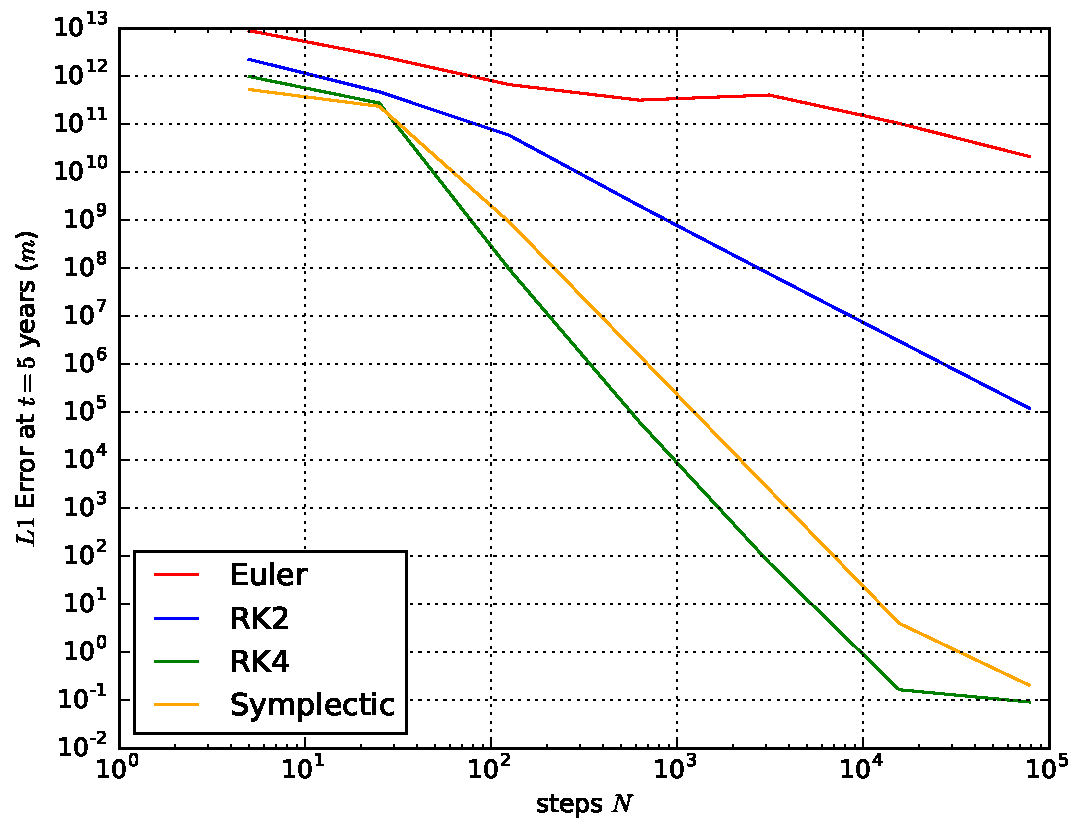
\includegraphics[width=\textwidth,keepaspectratio]{1_error}
              \caption{$L_1$ error as function of steps}
      \end{figure}
  \end{column}
  \begin{column}{.5\textwidth}
        \centering
        \begin{figure}
        \centering
      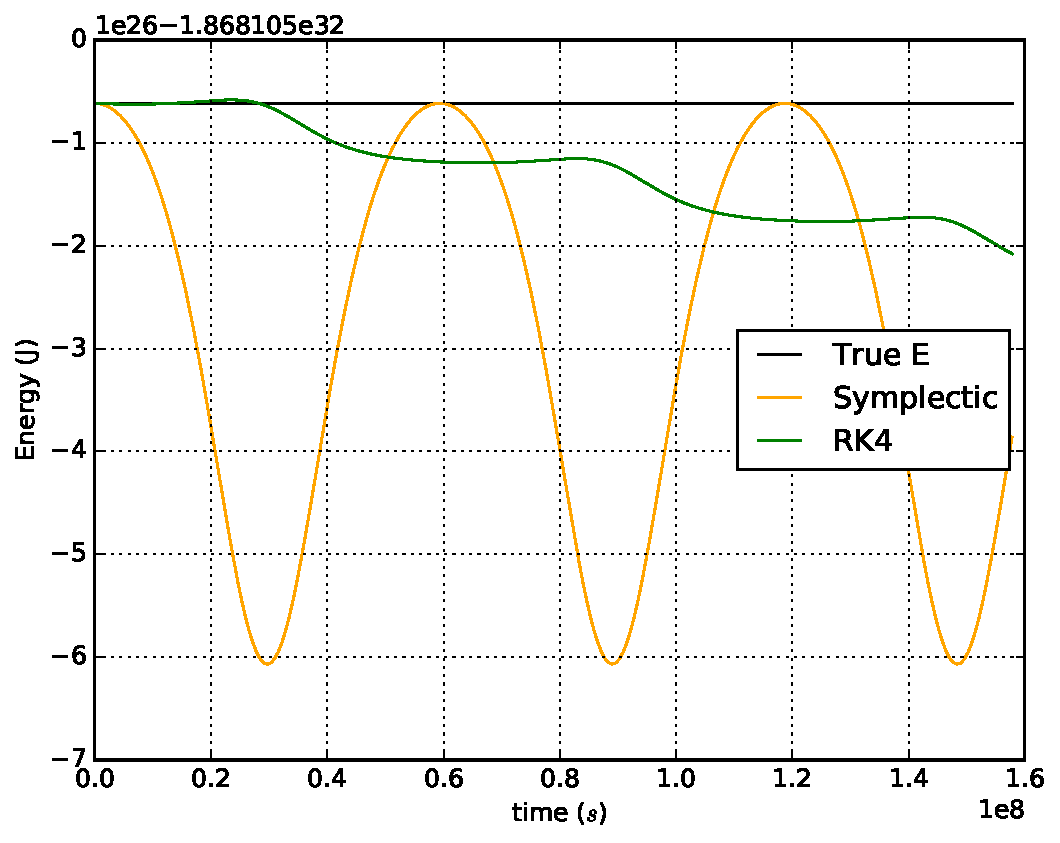
\includegraphics[width=\textwidth,keepaspectratio]{1_rk4_energy}
              \caption{Total energy over time}
      \end{figure}
  \end{column}
\end{columns}
\end{frame}

\begin{frame}{Performance}
  \begin{itemize}
    \item Need to support $1000+$ particles
    \item Performance bottleneck: force between each particle
    \item How to calculate force between every particle?
    \begin{itemize}
    \item[\xmark] Loop over them in Python
    \begin{itemize}
      \item This supported at most 50 particles, took half a day to run small timescale
    \end{itemize}
    \item[\cmark] Use \texttt{numpy} to eliminate loops entirely by doing all operations on \texttt{numpy} arrays
  \end{itemize}
  \item Use multi-threaded libraries to rewrite \texttt{numpy} code to be parallel
  \item Final performance: Simulation of collision runs with 2020 particles in about an hour
  \end{itemize}
\end{frame}

\begin{frame}{Visualization and Conclusion}
  \begin{itemize}
    \item Data visualization was done in \texttt{matplotlib}
    \item Animated the collision and rendered to video
    \item Animation is on \href{https://www.youtube.com/watch?v=Qp0M3gj23YY}{\beamergotobutton{YouTube}}
\\~\\
\begin{center}
\huge Questions?
\end{center}
  \end{itemize}
  
\end{frame}

\end{document}